\documentclass[12pt]{article}
\usepackage[utf8]{inputenc}
\usepackage{float}
\usepackage{amsmath}


\usepackage[hmargin=3cm,vmargin=6.0cm]{geometry}
%\topmargin=0cm
\topmargin=-2cm
\addtolength{\textheight}{6.5cm}
\addtolength{\textwidth}{2.0cm}
%\setlength{\leftmargin}{-5cm}
\setlength{\oddsidemargin}{0.0cm}
\setlength{\evensidemargin}{0.0cm}

%misc libraries goes here
\usepackage{tikz}
\usetikzlibrary{automata,positioning}

\begin{document}

\section*{Student Information } 
%Write your full name and id number between the colon and newline
%Put one empty space character after colon and before newline
Full Name : Beyazıt Yalçınkaya \\
Id Number : 2172138 \\

% Write your answers below the section tags
\section*{Answer 1}

\subsection*{a.}
A pushdown automaton for bottom-up parser of $G = (V, \Sigma, R, S)$ is defined as follows. $M = (K, \Sigma, \Gamma, \Delta, s, F)$, where
\begin{itemize}
	\item $K = \{p, q\}$,
	\item $\Sigma = \{a, b, c\}$,
	\item $\Gamma = \{a, b, c, S, X\}$,
	\item $\Delta = \{((p, a, e), (p, a)), ((p, b, e), (p, b)), ((p, c, e), (p, c)), ((p, e, XaXSa), (p, S)),\\ ((p, e, XbXSb), (p, S)), ((p, e, c), (p, S)), ((p, e, Xa), (p, X)), ((p, e, Xb), (p, X)),\\ ((p, e, e), (p, X)), ((p, e, S), (q, e))\}$,
	\item $s = p$, and
	\item $F = \{q\}$
\end{itemize}

\subsection*{b.}
\begin{equation*}
\begin{split}
	(p, abbcbabbaa, e) & \vdash_M (p, bbcbabbaa,   a)\\
				       & \vdash_M (p, bcbabbaa,   ba)\\
				       & \vdash_M (p, cbabbaa,   bba)\\
				       & \vdash_M (p, babbaa,   cbba)\\
				       & \vdash_M (p, babbaa,   Sbba)\\
				       & \vdash_M (p, babbaa,  XSbba)\\
				       & \vdash_M (p, abbaa,  bXSbba)\\
				       & \vdash_M (p, abbaa, XbXSbba)\\
				       & \vdash_M (p, abbaa,     Sba)\\
				       & \vdash_M (p, bbaa,     aSba)\\
				       & \vdash_M (p, bbaa,    XaSba)\\
				       & \vdash_M (p, bbaa,     XSba)\\
				       & \vdash_M (p, baa,     bXSba)\\
				       & \vdash_M (p, baa,    XbXSba)\\
				       & \vdash_M (p, baa,        Sa)\\
				       & \vdash_M (p, aa,        bSa)\\
				       & \vdash_M (p, a,        abSa)\\
				       & \vdash_M (p, a,       XabSa)\\
				       & \vdash_M (p, a,        XbSa)\\
				       & \vdash_M (p, a,         XSa)\\
				       & \vdash_M (p, e,        aXSa)\\
				       & \vdash_M (p, e,       XaXSa)\\
				       & \vdash_M (p, e,           S)\\
				       & \vdash_M (q, e,           e)
\end{split}
\end{equation*}



\section*{Answer 2}

\subsection*{a.}
%Do not submit solutions for b, yet solve it to prepare for the final.
Formal description for the Turing machine that computes the function $f$ is given as follows.

$M = (K, \Sigma, \delta, s, H)$ where,
\begin{itemize}
	\item $K = \{q_0, q_{Even}, q_{Odd}, q_{MarkGoLeft}, q_{MarkGoRight}, q_{Begin}, q_{End}, q_{PutOnes}, q_{DelteMarks}, h\}$,
	\item $\Sigma = \{\sqcup, \triangleright, 1, \#\}$,
	\item $\delta$ is given in Table~\ref{table:delta} (Note that, due to the constraint on the input strings and implementation of the machine some of the transitions can never be enabled, for the sake of simplicity those transitions are omitted in the table.),
	\item $s = q_0$, and
	\item $H = \{h\}$.
\end{itemize}


\begin{table}[H]\caption{$\delta$ function}\label{table:delta}
\begin{center}
\begin{tabular}{ | c | c | c | }
\hline
$q$ & $\sigma$ & $\delta(q, \sigma)$\\
\hline
$q_0$ & $\sqcup$ & $(q_{Even}, \sqcup, \rightarrow)$\\
%\hline
%$q_0$ & $\triangleright$ & $(q_0, \triangleright, \rightarrow)$\\
%\hline
%$q_0$ & $1$ & $(q_{0}, 1, \rightarrow)$\\
%\hline
%$q_0$ & $\#$ & $(q_{0}, \#, \rightarrow)$\\
\hline
$q_{Even}$ & $\sqcup$ & $(q_{MarkGoLeft}, \sqcup, \leftarrow)$\\
%\hline
%$q_{Even}$ & $\triangleright$ & $(q_{Even}, \triangleright, \rightarrow)$\\
\hline
$q_{Even}$ & $1$ & $(q_{Odd}, 1, \rightarrow)$\\
%\hline
%$q_{Even}$ & $\#$ & $(q_{Trap}, \#, \rightarrow)$\\
\hline
$q_{Odd}$ & $\sqcup$ & $(h, 1, \rightarrow)$\\
%\hline
%$q_{Odd}$ & $\triangleright$ & $(q_{Odd}, \triangleright, \rightarrow)$\\
\hline
$q_{Odd}$ & $1$ & $(q_{Even}, 1, \rightarrow)$\\
%\hline
%$q_{Odd}$ & $\#$ & $(q_{Trap}, \#, \rightarrow)$\\
%\hline
%$q_{MarkGoLeft}$ & $\sqcup$ & $(q_{MarkGoLeft}, \sqcup, \rightarrow)$\\
%\hline
%$q_{MarkGoLeft}$ & $\triangleright$ & $(q_{MarkGoLeft}, \triangleright, \rightarrow)$\\
\hline
$q_{MarkGoLeft}$ & $1$ & $(q_{Begin}, \#, \leftarrow)$\\
\hline
$q_{MarkGoLeft}$ & $\#$ & $(q_{PutOnes}, 1, \leftarrow)$\\
%\hline
%$q_{MarkGoRight}$ & $\sqcup$ & $(q_{MarkGoRight}, \sqcup, \rightarrow)$\\
%\hline
%$q_{MarkGoRight}$ & $\triangleright$ & $(q_{MarkGoRight}, \triangleright, \rightarrow)$\\
\hline
$q_{MarkGoRight}$ & $1$ & $(q_{End}, \#, \rightarrow)$\\
%\hline
%$q_{MarkGoRight}$ & $\#$ & $(q_{MarkGoRight}, \#, \rightarrow)$\\
\hline
$q_{Begin}$ & $\sqcup$ & $(q_{MarkGoRight}, \sqcup, \rightarrow)$\\
%\hline
%$q_{Begin}$ & $\triangleright$ & $(q_{Begin}, \triangleright, \rightarrow)$\\
\hline
$q_{Begin}$ & $1$ & $(q_{Begin}, 1, \leftarrow)$\\
\hline
$q_{Begin}$ & $\#$ & $(q_{MarkGoRight}, \#, \rightarrow)$\\
%\hline
%$q_{End}$ & $\sqcup$ & $(q_{MarkGoLeft}, \sqcup, \leftarrow)$\\
%\hline
%$q_{End}$ & $\triangleright$ & $(q_{End}, \triangleright, \rightarrow)$\\
\hline
$q_{End}$ & $1$ & $(q_{End}, 1, \rightarrow)$\\
\hline
$q_{End}$ & $\#$ & $(q_{MarkGoLeft}, \#, \leftarrow)$\\
\hline
$q_{PutOnes}$ & $\sqcup$ & $(q_{DeleteMarks}, \sqcup, \rightarrow)$\\
%\hline
%$q_{PutOnes}$ & $\triangleright$ & $(q_{PutOnes}, \triangleright, \rightarrow)$\\
%\hline
%$q_{PutOnes}$ & $1$ & $(q_{Trap}, 1, \rightarrow)$\\
\hline
$q_{PutOnes}$ & $\#$ & $(q_{PutOnes}, 1, \leftarrow)$\\
\hline
$q_{DeleteMarks}$ & $\sqcup$ & $(h, \sqcup, \rightarrow)$\\
%\hline
%$q_{DeleteMarks}$ & $\triangleright$ & $(q_{DeleteMarks}, \triangleright, \rightarrow)$\\
\hline
$q_{DeleteMarks}$ & $1$ & $(q_{DeleteMarks}, 1, \rightarrow)$\\
\hline
$q_{DeleteMarks}$ & $\#$ & $(q_{DeleteMarks}, \sqcup, \rightarrow)$\\
\hline
\end{tabular}
\end{center}
\end{table}

\section*{Answer 3}
The set of languages that is decided by Move-restricted Turing Machines is the set of regular languages. Even though Move-restricted Turing Machines are able to write on the input tape since they cannot move their head left, they do not have any memory, so they can only read the input once and make computations accordingly. This makes them equivalent to finite state automata and it is known that the set of languages accepted by finite state automata is the set of regular languages. Hence, the set of languages decided by Move-restricted Turing Machines is the set of regular languages.

\section*{Answer 4}

\subsection*{a.}
A Queue-based deterministic Turing Machine is a tuple $(K, \Sigma, \delta, s, F)$, where
\begin{itemize}
	\item $K$ is a finite set of states,
	\item $\Sigma$ is an alphabet (the input symbols),
	\item $s \in K$ is the initial state,
	\item $F \subseteq K$ is the set of final states, and
	\item $\delta: K \times \Sigma \to K \times \Sigma^*$ is the transition function.
\end{itemize}

\subsection*{b.}
A configuration of a Queue-based deterministic Turing Machine $M = (K, \Sigma, \delta, s, H)$ is a member of $K \times \Sigma^*$: The first component is the state of the machine, the second component is the contents of the queue, read from front to rear. Notice that for a Queue-based deterministic Turing Machine, it is assumed that the queue initially contains the input string so we use same alphabet for input and queue.

\subsection*{c.}
If $(p, \alpha\beta)$ and $(q, \beta\gamma)$ are configurations of $M$, we say that $(p, \alpha\beta)$ yields in one step $(q, \beta\gamma)$ \big(notation: $(p, \alpha\beta) \vdash_M (q, \beta\gamma)$\big) if there is a transition $\delta(p, \alpha) = (q, \gamma)$. We denote the reflexive, transitive closure of $\vdash_M$ as $\vdash_M^*$. We assume that the front and rear heads initially point to the beginning and end of the input string, that is queue initially contains the input string. The language accepted by $\vdash_M^*$ (which is the language accepted by $M$) denoted in set notation as follows.
\begin{align}
	L(M) = \{w \in \Sigma^* \mid (s, w) \vdash_M^* (f, e) \text{ for the initial state } s \text{ and for some } f \in F\}
\end{align}

\subsection*{d.}
To prove that the queue-based deterministic TM is equivalent to the standard TM, we provide a one-to-one mapping between the operations of two machines.

\noindent Below, we list the mapping from the standard TM to the queue-based TM.
\begin{itemize}
	\item To go left in the standard TM, it is necessary to enqueue read symbols while properly marking the needed positions of the queue with special symbols and then dequeue until the marking symbols to reach desired position in the queue-based TM.
	\item To go right in the standard TM, it is necessary to dequeue (while enqueuing needed symbols to not lose them for the other parts of the computation, if necessary) in the queue-based TM.
	\item To write a symbol on tape in the standard TM, it is necessary to enqueue in the queue-based TM.
	\item To read a symbol on tape in the standard TM, it is necessary to just check the symbol at the front  in the queue-based TM. 
\end{itemize}

\noindent Below, we list the mapping from the queue-based TM to the standard TM.
\begin{itemize}
	\item To access the front element in the queue-based TM, it is necessary to go first symbol in the tape and read it in the standard TM.
	\item To access the rear element in the queue-based TM, it is necessary to go last symbol in the tape and read it in the standard TM.
	\item To enqueue in the queue-based TM, it is necessary to add desired symbol after the last symbol of the input tape in the standard TM.
	\item To dequeue in the queue-based TM, it is necessary to write blank symbol onto the first symbol of the input tape in the standard TM.
\end{itemize}

\noindent This completes the proof. Hence, the queue-based deterministic TM is equivalent to the standard TM.
\subsection*{e.}
We formally define a queue-based deterministic TM $M$ such that $L(M) = L$ where $L = \{wcw \colon w \in \{a, b\}^*\}$ as follows. $M = (K, \Sigma, \delta, s, F)$, where
\begin{itemize}
	\item $K = \{q_0, q_1, q_2, q_3, q_4, y, n\}$,
	\item $\Sigma = \{a, b, c\}$,
	\item $\delta$ is given in Tab.~\ref{table:delta_queue},
	\item $s = q_0$, and
	\item $F = \{y, n\}$.
\end{itemize}

\begin{table}[H]\caption{$\delta$ function}\label{table:delta_queue}
\begin{center}
\begin{tabular}{ | c | c | c | }
\hline
$q$ & $\sigma$ & $\delta(q, \sigma)$\\
\hline
$q_0$ & $a$ & $(q_1, c)$\\
\hline
$q_0$ & $b$ & $(q_2, c)$\\
\hline
$q_0$ & $c$ & $(y, e)$\\
\hline
$q_1$ & $a$ & $(q_1, a)$\\
\hline
$q_1$ & $b$ & $(q_1, b)$\\
\hline
$q_1$ & $c$ & $(q_3, e)$\\
\hline
$q_2$ & $a$ & $(q_2, a)$\\
\hline
$q_2$ & $b$ & $(q_2, b)$\\
\hline
$q_2$ & $c$ & $(q_4, e)$\\
\hline
$q_3$ & $a$ & $(q_0, e)$\\
\hline
$q_3$ & $b$ & $(n, e)$\\
\hline
$q_3$ & $c$ & $(n, e)$\\
\hline
$q_4$ & $a$ & $(n, e)$\\
\hline
$q_4$ & $b$ & $(q_0, e)$\\
\hline
$q_4$ & $c$ & $(n, e)$\\
\hline

\end{tabular}
\end{center}
\end{table}






\section*{Answer 5}

\subsection*{a.}
Notice that for the machine given below, it is assumed that initially, the input is always in the following form: $\triangleright \underline{\sqcup} w \sqcup$ for some $w \in \{a, b, c\}^*$. The notation in the book has been adopted and basic machines defined in the book are used such as $R, L, R_{\sqcup}, L_{\sqcup}$.

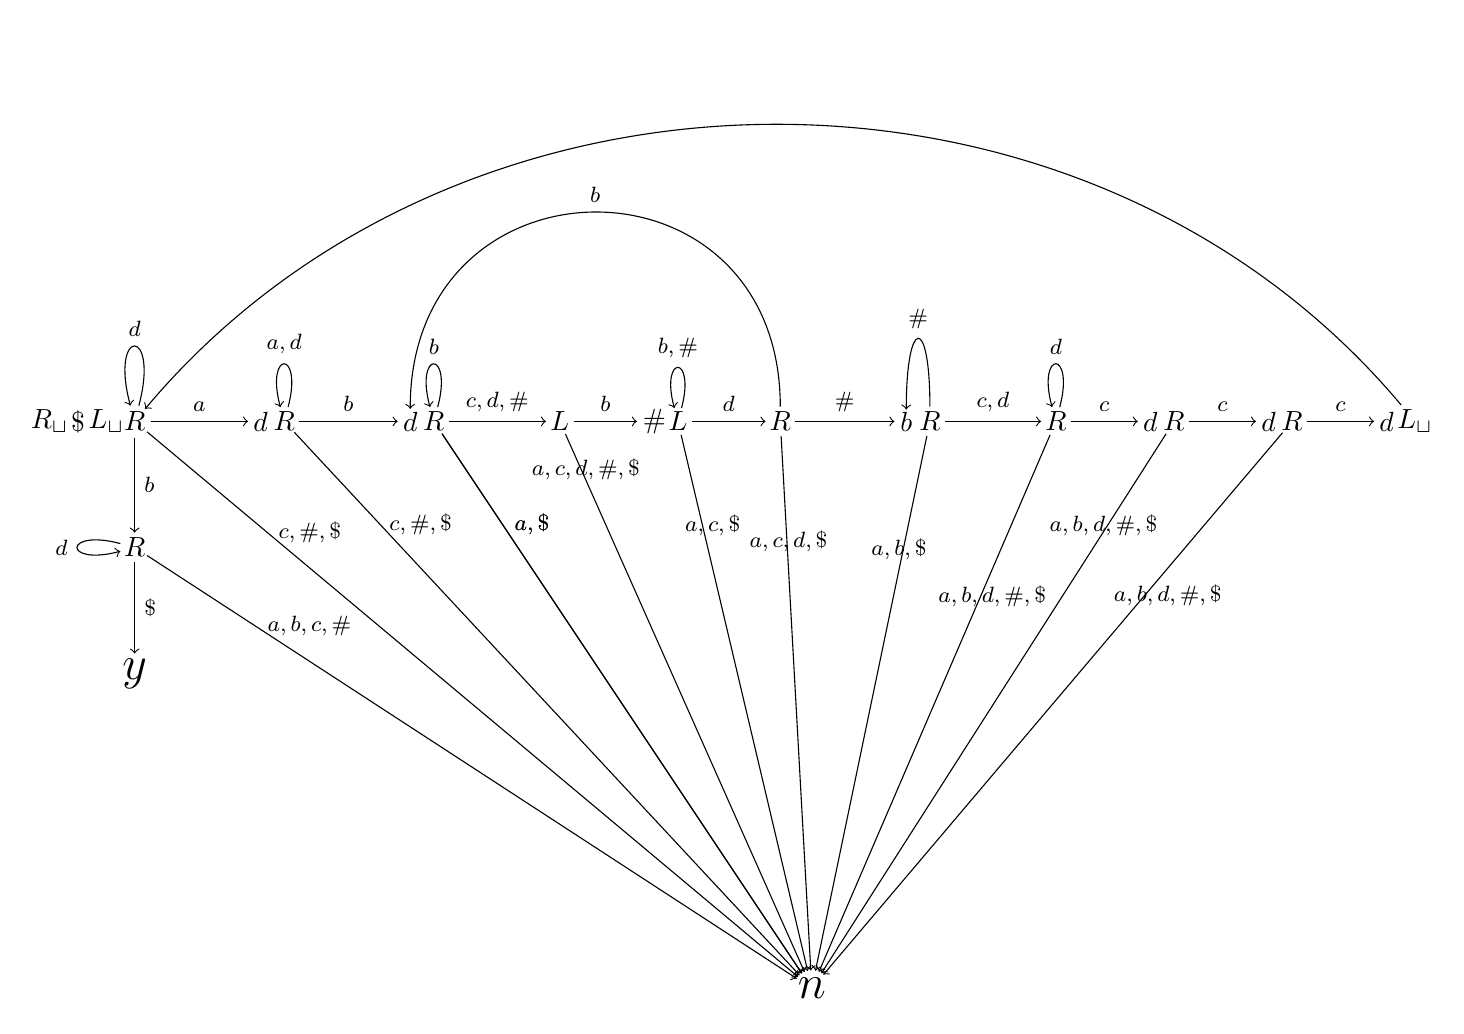
\begin{tikzpicture}[node distance=1.6cm, on grid, auto]

%\node[state, draw = none, fill = none, minimum size=4mm, inner sep=0pt] (x) {$R$};
\node[state, draw = none, fill = none, node distance =1.2 cm, minimum size=4mm, inner sep=0pt] (y) {$R_{\sqcup}$};
\node[state, draw = none, fill = none, right of = y, node distance =0.36 cm,  minimum size=4mm, inner sep=0pt] (z) {$\$$};
\node[state, draw = none, fill = none, right of = z, node distance =0.36 cm,  minimum size=4mm, inner sep=0pt] (t) {$L_{\sqcup}$};
\node[state, draw = none, fill = none, right of = t, node distance =0.36 cm,  minimum size=4mm, inner sep=0pt] (q_0) {$R$};
\node[state, draw = none, fill = none, below of = q_0, minimum size=2mm, inner sep=0pt] (q_1) {$R$};
\node[state, draw = none, fill = none, right of = q_0, minimum size=2mm, inner sep=0pt] (q_2) {$d$};
\node[state, draw = none, fill = none, right of = q_2, node distance =0.3 cm, minimum size=2mm, inner sep=0pt] (q_3) {$R$};
\node[state, draw = none, fill = none, right of = q_3, minimum size=2mm, inner sep=0pt] (q_4) {$d$};
\node[state, draw = none, fill = none, right of = q_4, node distance =0.3 cm, minimum size=2mm, inner sep=0pt] (q_5) {$R$};
\node[state, draw = none, fill = none, right of = q_5, node distance =1.6 cm, minimum size=2mm, inner sep=0pt] (q_6) {$L$};
\node[state, draw = none, fill = none, right of = q_6, node distance =1.2 cm, minimum size=2mm, inner sep=0pt] (q_7) {$\#$};
\node[state, draw = none, fill = none, right of = q_7, node distance =0.3 cm, minimum size=2mm, inner sep=0pt] (q_8) {$L$};
\node[state, draw = none, fill = none, right of = q_7, minimum size=2mm, inner sep=0pt] (q_8_1) {$R$};
\node[state, draw = none, fill = none, right of = q_8_1, minimum size=2mm, inner sep=0pt] (q_9) {$b$};
\node[state, draw = none, fill = none, right of = q_9, node distance =0.3 cm, minimum size=2mm, inner sep=0pt] (q_10) {$R$};
\node[state, draw = none, fill = none, right of = q_10, minimum size=2mm, inner sep=0pt] (q_11) {$R$};
\node[state, draw = none, fill = none, right of = q_11, node distance =1.2 cm, minimum size=2mm, inner sep=0pt] (q_12) {$d$};
\node[state, draw = none, fill = none, right of = q_12, node distance =0.3 cm, minimum size=2mm, inner sep=0pt] (q_13) {$R$};
\node[state, draw = none, fill = none, right of = q_13, node distance =1.2 cm, minimum size=2mm, inner sep=0pt] (q_14) {$d$};
\node[state, draw = none, fill = none, right of = q_14, node distance =0.3 cm, minimum size=2mm, inner sep=0pt] (q_15) {$R$};
\node[state, draw = none, fill = none, right of = q_15, node distance =1.2 cm, minimum size=2mm, inner sep=0pt] (q_16) {$d$};
\node[state, draw = none, fill = none, right of = q_16, node distance =0.36 cm, minimum size=2mm, inner sep=0pt] (q_17) {$L_{\sqcup}$};
\node[state, draw = none, fill = none, below of = q_1, minimum size=2mm, inner sep=0pt] (yes) {\LARGE$y$};
\node[state, draw = none, fill = none, right of = yes, xshift = 5 cm, minimum size=2mm, inner sep=0pt, xshift = 2 cm, yshift = -4 cm] (no) {\LARGE$n$};

\path[->]
(q_0) edge [out=75, in=105, looseness=25] node [above] {\footnotesize$d$}  (q_0)
(q_0) edge node {\footnotesize$b$} (q_1)
(q_1) edge node {\footnotesize$\$$} (yes)
(q_0) edge node {\footnotesize$a$} (q_2)
(q_3) edge [out=75, in=105, looseness=20] node [above] {\footnotesize$a, d$}  (q_3)
(q_3) edge node {\footnotesize$b$} (q_4)
(q_5) edge [out=75, in=105, looseness=20] node [above] {\footnotesize$b$}  (q_5)
(q_5) edge node {\footnotesize$c, d, \#$} (q_6)
(q_8) edge [out=75, in=105, looseness=20] node [above] {\footnotesize$b, \#$}  (q_8)
(q_8) edge node {\footnotesize$d$}  (q_8_1)
(q_8_1) edge node {\footnotesize$\#$}  (q_9)
(q_8_1) edge [out=90, in=90, looseness=1.8] node [above] {\footnotesize$b$}  (q_4)
(q_10) edge [out=90, in=90, looseness=10] node [above] {\footnotesize$\#$}  (q_9)
(q_10) edge node [above] {\footnotesize$c, d$}  (q_11)
(q_11) edge [out=75, in=105, looseness=20] node [above] {\footnotesize$d$}  (q_11)
(q_11) edge node [above] {\footnotesize$c$}  (q_12)
(q_13) edge node [above] {\footnotesize$c$}  (q_14)
(q_15) edge node [above] {\footnotesize$c$}  (q_16)
(q_17) edge [out=130, in=50, looseness=1] node [above] {}  (q_0)
(q_1) edge [out=165, in=195, looseness=20] node [left] {\footnotesize$d$}  (q_1)
(q_6) edge node {\footnotesize$b$} (q_7)


(q_0) edge node [near start, above, yshift = 2mm] {\footnotesize$c, \#, \$$} (no)
(q_1) edge node [near start, above, yshift = 2mm] {\footnotesize$a, b, c, \#$} (no)
(q_3) edge node [near start, above, yshift = 3mm] {\footnotesize$c, \#, \$$} (no)
(q_5) edge node [near start, above, yshift = 3mm] {\footnotesize$a, \$$} (no)
(q_5) edge node [near start, above, yshift = 3mm] {\footnotesize$a, \$$} (no)
(q_6) edge node [near start, above, yshift = 10mm, xshift = -5mm] {\footnotesize$a, c, d, \#, \$$} (no)
(q_8) edge node [near start, above, yshift = 3mm] {\footnotesize$a, c, \$$} (no)
(q_8_1) edge node [near start, above, yshift = 1mm] {\footnotesize$a, c, d, \$$} (no)
(q_10) edge node [near start, above, yshift = 0mm] {\footnotesize$a, b, \$$} (no)
(q_11) edge node [near start, above, yshift = -6mm] {\footnotesize$a, b, d, \#, \$$} (no)
(q_13) edge node [near start, above, yshift = 3mm, xshift = 3mm] {\footnotesize$a, b, d, \#, \$$} (no)
(q_15) edge node [near start, above, yshift = -6mm] {\footnotesize$a, b, d, \#, \$$} (no)
%(x) edge node [above] {$a, b$}  (y)
%(y) edge node [above] {$\sqcup$}  (z)
%(t) edge node [above] {$\sqcup$}  (q_0)

;
\end{tikzpicture}


\subsection*{b.}

We formally define a grammar $G$ such that $L(G) = L$ where $L = \{a^nb^{2^n}c^{3n} \colon n \in \mathbf{N}\}$ as follows, $G = (\{a, b, c, S, S', T, G, B, C, \$\}, \{a, b, c\}, R, S)$, where $R$ is given below.
\begin{equation}
\begin{split}
	S & \rightarrow aTBBCCC\$ \mid b \\
	S' & \rightarrow aTGCCC \\
	GB & \rightarrow BBG \\
	GC & \rightarrow CG \\
	G\$ & \rightarrow \$ \\
	aTB & \rightarrow aS'B \mid aB \\
	CB & \rightarrow BC \\
	aB & \rightarrow ab \\
	bB & \rightarrow bb \\
	bC & \rightarrow bc \\
	cC & \rightarrow cc \\
	c\$ & \rightarrow c
\end{split}
\end{equation}



\section*{Answer 6}

\subsection*{a.}

\begin{itemize}
\item Since $L_1$ can be generated by a regular grammar, it is a regular language. Since each regular language is accepted by some finite automaton, $L_1$ is accepted by some finite automaton. Any finite automaton can be mimicked by a Turning Machine, then, trivially, there exists a Turing Machine $M_1$ that accepts $L_1$.
\item The information "A deterministic top-down parser can be built for context-free grammar whose language is $L_2$" implies that there exists a deterministic pushdown automaton that accepts $L_2$. Since any deterministic pushdown automaton can be mimicked by a Turning Machine,  there exists a Turing Machine $M_2$ that accepts $L_2$.
\item Even though it is ambiguous, a context-free grammar can provide $L_3$, then there exists a pushdown automaton that accepts $L_3$. Since any pushdown automaton can be mimicked by a Turning Machine,  there exists a Turing Machine $M_3$ that accepts $L_3$.
\item Since there is a Turing Machine that decides $\overline{L_4} \cap \overline{L(a^*b^*)}$, $\overline{L_4} \cap \overline{L(a^*b^*)}$ is a recursive language. If $L$ is a recursive language, then its complement $\overline{L}$ is also recursive (Elements of Theory of Computation, page 199, Theorem 4.2.1), then $\overline{\overline{L_4} \cap \overline{L(a^*b^*)}} = L_4 \cup L(a^*b^*)$ is also recursive. $L(a^*b^*)$ is a regular language, then it is trivially recursive. Since a nondeterministic Turing Machine can be easily constructed for union of two recursive languages and it is know that nondeterministic Turing Machines are equivalent to deterministic Turing Machines, recursive languages are closed under union. Then since $L_4 \cup L(a^*b^*)$ and $L(a^*b^*)$ are recursive, $L_4$ is also a recursive language. Then there exists a Turning Machine $M_4$ that accepts $L_4$.
\item A language is generated by a grammar if and only if it is recursively enumerable (Elements of Theory of Computation, page 229, Theorem 4.6.1), then $L_5$ is a recursively enumerable language. A language is recursively enumerable if and only if there is a Turing Machine that semidecides it (Elements of Theory of Computation, page 198, Definition 4.2.4), then there exists a Turing Machine $M_5$ that accepts $L_5$.
\end{itemize}

\subsection*{b.}
\begin{itemize}
\item As it is argued in part a, $L_1$ is a regular language. Regular languages are subset of recursive languages in Chomsky hierarchy, then $L_1$ can be considered as a recursive language. For any recursive language there exists a Turning Machine that decides it, meaning a decider can be constructed for $L_1$ for membership problems. Hence there is always an algorithm for membership problems associated with $L_1$.
\item As it is argued in part a, $L_2$ is a deterministic context-free language, then it is trivially a context-free language. Same argument as above applies for $L_2$, too. Thus, there is always an algorithm for membership problems associated with $L_2$.
\item As it is argued in part a, $L_3$ is a context-free language. Same argument as above applies for $L_3$, too. Thus, there is always an algorithm for membership problems associated with $L_3$.
\item As it is argued in part a, $L_4$ is a recursive language. For any recursive language there exists a Turning Machine that decides it. Thus, there is always an algorithm for membership problems associated with $L_3$.
\item As it is argued in part a, $L_5$ is a recursively enumerable language. There are recursively enumerable languages for which there is no TM that decides them. Thus, we cannot say that there is always an algorithm for membership problems associated with $L_5$, in some cases there is and in some cases there is no such algorithm. 
\end{itemize}

\subsection*{c.}
To show this, we define the following machines. Notice that we assume any given input $w \in \Sigma^*$, where $\Sigma$ is the alphabets of the machines, the tape is in the following form: $\triangleright \sqcup w \sqcup$. As it is argued in part b, there exists deciders for $L_1$, $L_2$, $L_3$, and $L_4$. Say machines $M_1$, $M_2$, $M_3$, and $M_4$ are deciders, i.e. they halt on any given input. Define two TMs $\overline{M_2}$ that accepts $\overline{L_2}$ and $\overline{M_4}$ that accepts $\overline{L_4}$. Those machines can be easily defined, just switch halting states of the original machines, i.e. say $y$ is $n$ and $n$ is $y$. Define another TM $M_x$ as follows: Operate as $\overline{M_2}$ if it halts on $n$ for the given string then halt on $n$, else if it halts on $y$ then for rest of the string operate as $M_1$. $M_x$ accepts the language $\overline{L_2}L_1$.  Define a TM $M_y$ that halts on $y$ for a given string if and only if both $M_x$ and $M_5$ halt on $y$ for the same string. Notice that $M_y$ semidecides the language $\overline{L_2}L_1 \cap L_5$. Define $M_y^*$ in basic machines notation as follows.
\begin{center}
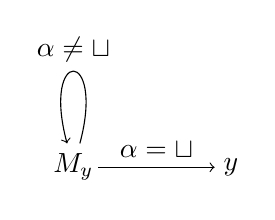
\begin{tikzpicture}[node distance=2cm, on grid, auto]
\node[state, draw = none, fill = none, minimum size=4mm, inner sep=0pt] (q) {$M_y$};
\node[state, draw = none, fill = none, right of = q, minimum size=4mm, inner sep=0pt] (p) {$y$};
\path[->]
(q) edge [out=75, in=105, looseness=20] node [above] {$\alpha \neq \sqcup$}  (q)
(q) edge node [above] {$\alpha = \sqcup$}  (p);
\end{tikzpicture}
\end{center}
Define a TM $M_3^*$ in a very similar manner as $M_y^*$ (it is omitted since it is almost the same as $M_y^*$).  Define a new TM $M_z$ in basic machines notation as follows.
\begin{equation*}
	M_3^* \rightarrow \overline{M_4}
\end{equation*}
Finally, we define a TM $M$ that accepts the given language $L$. $M$ halts on $y$ for a given string if and only if $M_y^*$ halts on $y$ for the given string or $M_z$  halts on $y$ for the given string. Notice that $M$ semidecides $L$. $M$ accepts any string in the given language $L$.
\subsection*{d.}
The TM $M$ defined for $L$ in part c semidecides $L$. We cannot always come up with a TM that semidecides $\overline{L}$.  When the machine does not halt for a string, we do not know whether the given string is not in the language or the machine is making a very long computation which will eventually accept the string, Since we cannot distinguish these two cases we cannot define a TM for $\overline{L}$. Notice that some TMs that semidecides their languages can be converted to a decider; however, there are TMs that cannot be converted into a decider. Due to this argument, it is known that recursively enumerable languages are not closed under complementation. Thus, we concluded that, we cannot always come up with a machine that semidecides $\overline{L}$.



%Do not submit solutions for Question 7, yet do solve it.


\end{document}

​

